%==================Kapitola: Kmitočtové filtry======================================================
\chapter{Kmitočtové filtry}
\minitoc
\newpage
  \section{Základní vlastnosti kmitočtových filtrů}
    \subsection{Kmitočtové filtry a jejich použití}
      Kmitočtové filtry jsou lineární elektrické obvody, používané v mnoha oblastech elektrotechniky
      a elektroniky. Jejich hlavním úkolem je \emph{výběr} (selekce) \emph{kmitočtových složek}
      procházejícího signálu podle jejich kmitočtů. Filtry obvykle nékteré kmitočtové složky signálů
      \emph{propouštějí} bez útlumu (oblast se nazývá propustným pásmem), jiné kmitočtové složky
      \emph{potlačují} (pásmo potlačeni, útlumu, nebo nepropustné pásmo). Tyto vlastnosti obvykle
      vyjadřujeme \emph{modulovou (amplitudovou) kmitočtovou charakteristikou} (závislost modulu
      napéťového přenosu na kmitočtu).

      Příklad použití kmitočtového filtru ukazuje názorně obr. \ref{aes:fig_KF_sedlacek_FiltrHP}.
      Užitečný obdélníkový signál byl znehodnocen nízkofrekvenční rušivou harmonickou složkou
      (pronikající např. z napájecí střídavé sítě - kmitočet sítě je nižší, než kmitočty užitečných
      složek), signál je označen v grafu jako \(u_1(t)\). Jak je z obrázku vidět, filtr typu horní
      propust propustil všechny kmitočtové složky s mezním kmitočtem vyšším než \(f_M\) (složky
      obdélníkového signálu) a potlačil tak nízkofrekvenční rušivou harmonickou složku, výsledný
      signál je v grafu označen jako \(u_2(t)\). Z obr \ref{aes:fig_KF_sedlacek_FiltrHP} je zřejmé,
      že vliv kmitočtových filtrů na signál je dobře patrný zvláště při znázornění procesu filtrace
      v kmitočtové oblasti pomoci kmitočtového spektra - tedy pomoci rozkladu signálu na jeho
      jednotlivé harmonické složky.

      Průchod signálu filtrem vede též obvykle k \emph{časovému zpožděni signálu}, což je důsledkem
      fázových posuvů (zpoždění) procházejících harmonických kmitočtových složek signálu. Tyto vlivy
      obvykle vyjadřujeme \emph{fázovou kmitočtovou charakteristikou}. Jejich vliv na výstupní
      signál je též zřejmý při znázornění signálu a vlastností filtru v \emph{časové oblasti} (např.
      odezva na jednotkový skok). Fázové vlivy filtru na signál v propustném kmitočtovém pásmu se v
      časové oblasti projevují např. jako nežádoucí překmity či zvlnění průběhu signálu. V příkladu
      z obr. \ref{aes:fig_KF_sedlacek_FiltrHP} (filtr typu horní propust) způsobil tento efekt
      zešikmení horních a spodních hran obdélníkového signálu. Uvedené vlivy je možné vhodnou
      volbou filtru minimalizovat. Na druhé straně ale existují případy, kdy těchto vlastností
      filtrů záměrné využíváme, např. ve fázovacích a zpožďovacích obvodech.

      \begin{figure}[ht!]
        \centering
        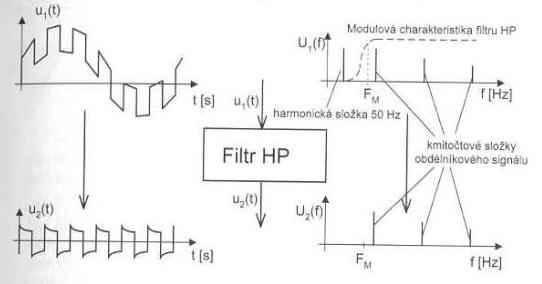
\includegraphics[width=0.8\linewidth]{KF_sedlacek_FiltrHP.jpg}
        \caption[Příklad filtru HP]{Příklad selekce kmitočtových složek signálu filtrem typu horní
                 propust pro potlačení nízkofrekvenční rušivé složky (např. kmitočet síté 50 Hz)}
        \label{aes:fig_KF_sedlacek_FiltrHP}    
      \end{figure} 
        
      \subsubsection{Oblasti a příklady použití kmitočtových filtrů}
        Kmitočtové filtry patří mezi základní stavební bloky pro zpracování signálů. V radiotechnice
        je časté použití pásmových propustí pro výběr přijímaných signálů (vstupní obvody přijímačů,
        mezifrekvenční filtry), dolních propustí a horních propustí jako výhybek pro rozdělení
        kmitočtových pásem v anténních obvodech a předzesilovačích, pásmových zádrží pro rejekci
        (potlačení) rušících signálů, dolních propustí pro různé typy demodulátorů atd. Moderní
        komunikační systémy s rozloženým spektrem vyžadují také jako jeden z důležitých bloků
        přijímače filtr typu pásmová propust. Obdobné je využití filtrů v telekomunikacích, při
        přenosu dat apod.
    
        V elektroakustice se velmi často využívají korekční filtry (nastavitelné korektory hloubek,
        výšek, pásmové korektory, korektory kmitočtových charakteristik dynamických přenosek,
        magnetofonových hlav), různé typy filtrů v systémech omezení šumu (Dolby apod ). Dolní,
        horní a pásmové propusti tvoří kmitočtové výhybky pro reproduktorové soustavy (pasivní i
        aktivní), jak ukazuje obr. \ref{aes:fig_KF_sedlacek_kmvhb}. V oblasti elektronické hudby se
        využívají i různé filtry pro zabarvení zvuku a realizaci zvláštních zvukových efektů.
      
        \begin{figure}[ht!]
          \centering
          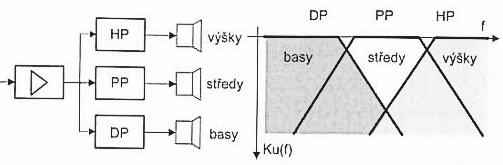
\includegraphics[width=0.8\linewidth]{KF_sedlacek_kmvhb.jpg}
          \caption[Příklad použití filtrů v kmitočtových výhybkách reproduktorových
                   soustav]{Příklad použití filtrů v kmitočtových výhybkách reproduktorových
                   soustav}
          \label{aes:fig_KF_sedlacek_kmvhb}    
        \end{figure} 
      
        Kmitočtové filtry se využívají také v oblasti \emph{měřicí techniky}. Velmi často jsou to
        filtry pro výběr měřeného kmitočtového pásma, obzvláště pak v různých typech selektivních
        měření (selektivní voltmetry, měřiče harmonického a dalších typů zkreslení, různá
        vysokofrekvenční měření). Pro akustická měření se využívá několika typů váhových filtrů pro
        měření úrovně akustického signálu (modeluje se vnímání lidského ucha). Často se využívá
        korektorů kmitočtových vlastností snímacích čidel. I přes rozvoj číslicových kmitočtových
        filtrů je výhodné u slabých a hodně zarušených signálů provést před A-D převodem analogovou
        předfiltraci pro podstatné zvýšení dynamického rozsahu systému.

        Zvláštní skupinu aplikací tvoří filtry typu dolní propust v systémech pro převod analogového
        signálu na číslicový. Pro splnění vzorkovacího teorému je zde v mnoha případech potřebné
        použit \emph{antialiasingový filtr} pro zamezení překládání rušivého spektra do užitečného
        signálu a na výstupu takového systému obdobný rekonstrukční filtr. Kmitočtové filtry se
        používají často v \emph{regulační technice}, speciální odrušovací filtry nacházejí uplatnění
        v \emph{silnoproudé elektrotechnice}. Takto bychom mohli vyjmenovat mnoho dalších aplikací.

        Lze říci, že neexistuje oblast elektrotechniky a elektroniky, kde se alespoň v omezené míře
        nevyužívají kmitočtové filtry. Základní orientace a znalost problematiky kmitočtových filtrů
        je proto potřebná prakticky pro každého tvůrčího pracovníka v elektrotechnice.
    
      \subsubsection{Způsoby realizací kmitočtových filtrů}
        Kmitočtové filtry můžeme v praxi realizovat mnoha odlišnými způsoby, které do určité míry
        určují i některé podstatné provozní vlastnosti filtru. Nejvhodnější způsob realizace je
        potřebné si pro daný účel optimálně vybrat. Tyto způsoby realizací lze rozdělit orientačně
         do tří hlavních skupin:
        \begin{itemize}
          \item Realizace z \textbf{diskrétních prvků} (odpory, kondenzátory, cívky, operační
                zesilovače apod), kde si každý uživatel může s menšími či většími problémy sestavit
                filtr přesné podle svých požadavků.
          \item Realizace v podobě \textbf{integrovaného bloku} je obvykle menší, levnější a lépe
                propracovaná, protože ji výrobce vyrábí ve velkých sériích vhodnou technologii. Na
                druhé straně si však uživatel obvykle nemůže upravit tento filtr podle svých
                speciálních požadavků a musí přesně dodržet podmínky zapojení podle výrobce.
          \item Realizace s \textbf{číslicovými filtry} spočívá v číslicovém zpracování signálu, kdy
                číslicovou interpretaci signálu matematicky upravujeme tak, aby výsledný signál měl
                po zpětném převodu shodné (či dokonce lepší) vlastnosti jako po průchodu normálním
                kmitočtovým filtrem. Matematicky tak modelujeme požadované vlastnosti filtrů a tímto
                způsobem lze dokonce realizovat i některé funkce a vlastnosti, které běžnými
                analogovými filtry nelze dosáhnout. Při realizaci jsme však omezeni na prostředí
                číslicového zpracování signálu (převodníky, počítač či signálový procesor, vhodný
                program). Značným omezením může být i maximální rychlost výpočtu počítače a
                vzorkování a tím i použitelné kmitočtové pásmo filtru.         
        \end{itemize}
        Jak je z tohoto dělení zřejmé, pro optimální výběr realizace filtru neexistuje univerzální
        návod, vždy záleží na podmínkách úlohy. Jde-li o úlohu, kdy řešíme číslicové zpracování
        signálu a máme dostatečnou výpočetní kapacitu daného prostředku, zvolíme číslicový filtr. V
        jiných případech (vysoký kmitočet signálů, slabý a zarušený signál, jde-li o výkonovou
        aplikaci apod.), použijeme analogový filtr. Při tomto řešení dáváme přednost standardnímu
        integrovanému filtru profesionální výroby (např. mezifrekvenční filtry přijímačů). Pokud
        však našim požadavkům plně nevyhovuje, musíme navrhnout a vyrobit filtr požadovaných
        vlastností z dostupných diskrétních součástek. Složitost a rozmanitost vlastností
        jednotlivých realizací filtrů ukazuje i jejich následující podrobnější přehled, který
        rozděluje jednotlivé typy filtrů podle použitých stavebních prvků:
        \begin{itemize}
          \item \textbf{Filtry RC} vynikají svou jednoduchostí, dostupností a nízkou cenou výchozích
                součástek, rezistorů a kondenzátorů. Plné však u nich platí:za málo penéz - málo
                muziky. Praktické využití mají jen jednoduché filtry prvního řádu a druhého řádu s
                nízkým činitelem jakosti (\(Q < \num{0.5}\)). Filtry RC vyšších řádů se v praxi
                používají výjimečně.
          \item \textbf{Filtry RLC} umožňují realizovat teoreticky libovolný typ filtru. Jejich
                omezeni vyplývá především z použití cívek. Ty jsou obzvláště pro nízké kmitočty
                (velké hodnoty L) rozměrné, drahé a ztrátové (malý činitel jakosti \(Q\)). Obecné je
                také použití filtrů RLC omezeno vlastními ztrátami cívek a kondenzátorů a také
                tolerancí a stabilitou jejich hodnot pro propusti a zádrže s velmi malou relativní
                šířkou pásma. Obvykle jsou používány v kmitočtovém rozsahu od \SI{100}{\kilo\hertz}
                do \SI{300}{\mega\hertz}, pro nižší kmitočty jen výjimečné. Pro kmitočty nad
                hranicí asi \SI{300}{\mega\hertz} se výrazné projevují parazitní vlastnosti prvků a
                je lépe využít realizaci s rozprostřenými parametry - viz následující bod.
          \item \textbf{Mikrovlnné filtry} jsou realizací RLC filtrů v oblasti mikrovln (\(f
                \SI{>>300}{\mega\hertz}\)), kde již nelze použít prvky se soustředěnými parametry
                (R, L, C), ale používá se odpovídající realizace s rozloženými parametry jako jsou
                vlnovody, mikropásková vedení, koaxiální vedeni apod.
          \item \textbf{Filtry ARC} (známé také jako \emph{aktivní filtry RC}) v principu nahrazují
                filtry RLC Místo cívek používají rezistory. kondenzátory a aktivní prvky, nejčastéji
                operační zesilovače. Mají obdobné vlastnosti jako filtry RLC. ale vzhledem k
                vlastnostem aktivních prvků se jejich použití omezuje nejčastéji na kmitočtové pásmo
                přibližné \SI{0.1}{\hertz} až \SI{100}{\kilo\hertz}. Současný pokrok v technologii
                aktivních prvků však umožňuje využití těchto filtrů na stále vyšších kmitočtech
                (dnes již řádové jednotky až desítky \si{\mega\hertz}), i když toto použití je zatím
                málo rozšířené. Kmitočtově jsou tedy vhodným doplňkem k filtrům RLC. Oproti nim mají
                výhodu i v snazší nastavitelnosti a laditelnosti změnou hodnot odporů. Jejich
                nevýhodou je na druhé straně potřeba napájení aktivních prvků. Objevují se i jejich
                specifické modifikace využívající parazitních vlastností aktivních prvků (R nebo C)
                jako stavebních prvků - filtry AC. AR apod.
          \item \textbf{Filtry ASC}, známé též jako \emph{filtry se spínanými kapacitory} jsou
                speciální modifikaci filtru ARC. které místo odporů používají přepínané
                kondenzátory. Jejich hlavní výhodou je možnost poměrně snadné monolitické integrace
                v porovnání s filtry ARC. Některé typy můžeme zakoupit jako integrované obvody.
                Jejich mezní kmitočet je určen spínacím kmitočtem a jsou tedy snadno přeladitelné.
                Lze je řadit již do skupiny integrovaných filtrů, nicméně jsou zde možnosti
                určitého přizpůsobení požadavkům, a to jednak přeladěním, jednak také dostupnosti
                integrovaných nastavitelných bloků 2. řádu. Na druhé straně je však tento typ
                realizace kmitočtově ještě více omezen než filtry ARC a má navíc problémy s vyšším
                driftem, s určitým průnikem spínacího signálu do užitečného signálu a
                „schodovitostí“ výsledného signálu, způsobenou spínáním. Spínací kmitočet bývá
                \(\num{50}\times\) až \(\num{100}\times\) vyšší než mezní kmitočet filtru, což do
                určité míry minimalizuje spínáním vzniklý projev diskretizace signálu v časové
                oblasti a možný aliasingový efekt (překládání spektra rušivého signálu do spektra
                užitečného signálu).
          \item \textbf{Elektromechanické filtry} jsou historicky nejstarší „integrované“ filtry.
                Vycházejí z principu převodu elektrického signálu na mechanický, využitím nékteré
                formy mechanické rezonance a zpětného převodu výsledného mechanického signálu na
                elektrický. Chovají se tedy vesměs jako pásmové propusti. Podle typu mechanického
                rezonátoru je lze dělit na různé skupiny. Dříve byly používány např. magnetostrikční
                filtry a dnes jsou používané nejčastěji \emph{piezokeramické filtry} (např.
                mezifrekvenčni filtry \SI{455}{\kilo\hertz} a \SI{10.7}{\mega\hertz}).
                Zvláštním typem je \emph{krystalový filtr}, který odpovídá v podstatě složenému
                rezonančnímu obvodu s vysokým činitelem jakosti (řádové \num{10000}) a vysokou
                stabilitou rezonančního kmitočtu. Nejčastěji se využívá ve stabilních oscilátorech.
                Vzhledem k vysokému a nenastavitelnému činiteli jakosti a nenastavitelnému
                rezonančnímu kmitočtu se krystaly jako filtry používají velmi omezené. Zapojením
                většího počtu krystalů s velmi přesným výběrem lze realizovat úzký pásmový filtr pro
                speciální aplikace jako např. úzkopásmové mezifrekvenčni filtry s vysokým
                rezonančním kmitočtem.
          \item \textbf{Filtry s PAV} (s \emph{povrchovou akustickou vlnou}, anglická zkratka SAW)
                jsou poměrné novým typem integrovaných filtrů, založených na principu vyzařování,
                šíření a fázového, kmitočtově závislého skládání povrchových akustických vln.
                Realizují se tak, že se nanese na nosnou keramickou destičku soustava vysílacích a
                přijímacích piezoelektrických zářičů, jejichž tvar a funkci lze přirovnat k dvěma
                Yagiho anténám. Obdobně jako u antén je rozměry a polohou zářičů tvarována přenosová
                kmitočtová charakteristika filtru. V porovnání s elektromechanickými filtry mohou
                realizovat podstatně širokopásmovéjší obvody. Proto se s výhodou používají, např.
                jako obrazové mezifrekvenčni filtry v televizorech a v mnoha dalších aplikacích pro
                vysoké kmitočty. Na druhou stranu je jejich použití částečné omezeno vyšším
                průchozím útlumem.
          \item \textbf{Filtry CCD} (\emph{charge coupled devices - nábojové vázané obvody}) jsou
                dalším speciálním typem aplikace s časové diskrétním charakterem (např. jako filtry
                ASC). Využívá se u nich technologie známá např. z CCD televizních kamer a princip
                spočívá v postupném posuvu a fázově závislém sčítání jednotlivých „nábojových
                vzorků“.
          \item \textbf{Číslicové filtry} jsou oproti předchozím filtrům odlišnou („softwarovou“)
                realizaci funkce filtrů, jejich princip byl popsán v předchozím odstavci.
        \end{itemize}
        Uvedený přehled potvrzuje značnou různorodost konečných realizací filtrů. Z přehledu
        vlastností jednotlivých typů kmitočtových filtrů je zřejmá i obtížnost úlohy konstruktéra
        při výběru optimálního způsobu realizace. Pro rychlejší orientaci o použitelnosti
        uvedených filtrů z hlediska kmitočtového pásma je možné využít tab.
        \ref{aes:fig_KF_sedlacek_kmtab}. Meze použití jednotlivých způsobů realizací je nutno chápat
        jen jako orientační, protože závisí nejen na současném stavu technologie, ale i na mnoha
        různých parametrech a požadavcích kladených na filtry.

        \begin{figure}[ht!]
          \centering
          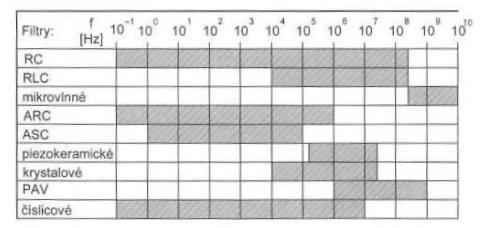
\includegraphics[width=0.8\linewidth]{KF_sedlacek_kmtab.jpg}
          \caption[Orientační znázornění kmitočtových pásem použitelnosti jednotlivých typů
                   realizaci filtrů]{Orientační znázornění kmitočtových pásem použitelnosti
                   jednotlivých typů realizaci filtrů}
          \label{aes:fig_KF_sedlacek_kmtab}    
        \end{figure} 
  
  \section{Popis přenosových vlastností filtrů, jejich charakteristiky}
    \subsection{Průchod signálu kmitočtovým filtrem a přenosové kmitočtové charakteristiky filtrů}
      Základní zapojeni filtru připojeného ke zdroji harmonického signálu je uvedeno na obr.
      \ref{aes:fig_KF_sedlacek_dvjbrn}. Procházi-li přes kmitočtový filtr harmonický signál s
      amplitudou \(U_1\), kmitočtem \(f_1\) a fázi \(\varphi_1\), získáme na výstupu filtru opět
      harmonický signál se stejným kmitočtem, ale jinou velikostí amplitudy a fáze (\(U_2\),
      \(\varphi_2\)).
  
      \begin{figure}[ht!]
        \centering
        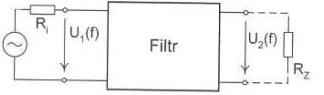
\includegraphics[width=0.8\linewidth]{KF_sedlacek_dvjbrn.jpg}
        \caption[Filtr jako dvojbran]{Filtr jako dvojbran}
        \label{aes:fig_KF_sedlacek_dvjbrn}    
      \end{figure}
      
      \textbf{Přenos napětí} \(\mathbb{K_U}\) harmonického signálu filtrem lze pro daný kmitočet
      \(f\) vyjádřit komplexním výrazem
      \begin{equation}\label{aes:eq_KF_ku}
        \mathbb{K_U} = K_U\cdot e^{j\varphi} = \frac{U_2e^{j\varphi_2}}{U_1e^{j\varphi_1}},
      \end{equation}
      který můžeme rozdělit na \emph{reálnou} a \emph{imaginární} část. Častěji ale používáme
      vyjádření přenosu pomocí \emph{modulu} a \emph{argumentu}
      \begin{equation}\label{aes:eq_KF_moarg}
        K_U = \frac{U_2}{U_1}, \qquad \varphi = \varphi_2 - \varphi_1, 
      \end{equation}
      kde modul \(K_U\) je poměr amplitud výstupního a vstupního signálu a argument \(\varphi\) je
      výsledný fázový posuv (časový rozdíl vztažený na periodu) mezi výstupním a vstupním signálem
      jako rozdíl fázi výstupního signálu \(\varphi_2\) a vstupního signálu \(\varphi_1\). Modul
      přenosu \(K_U\) je bezrozměrné číslo a často se udává v logaritmické míře, kdy platí \(K_U
      [\si{\decibel}] = 20 \log{K_U}\). Toto běžné používané vyjádření umožňuje grafické znázornění
      velkého rozsahu hodnot.
  
  \section{Přenosové vlastnosti a charakteristiky základních typů filtrů}
    \subsection{Filtry s přenosovou funkcí 1. řádu}
    \subsection{Filtry s přenosovou funkcí 2. řádu}
    \subsection{Přenosové funkce vyšších řádů}
    \subsection{Citlivost a tolerance přenosových vlastností filtrů} 
  \section{Návrh filtrů RC a RLC 1. a 2. řádu}
    \subsection{Návrh filtrů RC}
    \subsection{Návrh filtrů RLC 2. řádu}
    \subsection{Návrh fázovacích článků RLC 1. a 2. řádu}     
  \section{Filtry RLC vyšších řádů}
    
  \section{Filtry ARC 2. řádu}
    \subsection{Základní principy funkce filtrů ARC}
      Při realizaci filtrů RLC pro nízké kmitočty jsou největší problémy s kvalitou, rozměry a
      cenou cívek. Proto se pro nízké kmitočty s výhodou nahrazují \textbf{aktivními filtry RC}
      (filtry ARC). Jejich základní princip spočívá v "náhradě" cívky pomocí zapojení
      \emph{aktivního prvku} (operační zesilovač, tranzistor) se dvěma rezistory a kapacitory.
      Nahradit cívku můžeme v zásadě dvěma základními způsoby. První spočívá v použití obvodu,
      který přímo nahrazuje cívku jako dvojpól a vykazuje mezi určitými svorkami příslušnou
      indukčnost. Druhý princip, jak bude ukázáno dále, nahrazuje cívku nepřímo, pomoci
      transformace výchozího LRC obvodu na ekvivalentně se chovající strukturu RCD, která indukční
      prvek neobsahuje, ale na druhou stranu potřebuje \emph{syntetický prvek D} - dvojný kapacitor
      (kmitočtově závislý negativní rezistor).

    \subsection{Obvody s náhradou cívky}
      Aktivní filtry ARC, které vycházejí z filtru RLC a využívají k tomu přímou či nepřímou
      náhradu cívek, mají velké množství různých variant zapojeni. Objasnění jejich funkce
      představuje i řadu různých pohledů na činnost filtru. V oblasti návrhu ARC filtru převažují
      dva hlavni přístupy. Velmi názorný je takový přístup, který vytváří obvody, vykazující na
      vstupních svorkách induktivní impedanci. Ty lze využít jako přímou náhradu indukčnosti ve
      filtru RLC. Zřejmě nejčastější je ale takový pohled, kdy vytváříme celý obvod ARC s
      přenosovou funkci 2. řádu jako ekvivalenci obvodu LRC 2. řádu, přičemž přímá náhrada cívky v
      obvodu nemusí být na první pohled zřejmá.

    \subsection{Stavební prvky filtrů ARC a základní vlivy jejich reálných vlastností}
      Stavebními prvky filtrů ARC jsou rezistory, kapacitory a aktivní prvky, jak již bylo
      naznačeno v předešlém textu. I pro nejjednodušší posouzení funkce, klasifikaci a výběr
      optimálního zapojeni filtrů ARC je potřeba rozumět alespoň základním vlivům reálných
      vlastnosti těchto stavebních prvků na výsledné parametry ARC obvodu.

      \subsection{Vliv reálných odporů a kondenzátorů}
        ($C_1$, i $C_2$) vytvářejí se zbytkem obvodu rezonanční obvod RLC, lze vliv jejich ztrát
        modelovat sériovým či paralelním spojením ideálního kapacitoru s rezistorem. Tento vliv lze
        posuzovat v principu shodně jako u filtrů RLC. Při ideálních vlastnostech zbývající části
        obvodu určuje hodnotu činitele jakosti celkového obvodu činitel jakosti reálného
        kondenzátoru $Q_c = \frac{1}{tg\delta}$. Jeho hodnota musí být proto podstatně vyšší než
        výsledná funkční hodnota činitele jakosti celého obvodu (alespoň \(\num{10}\times\)). Při
        nižších hodnotách je třeba tento vliv brát v úvahu a pokud je to možné, kompenzujeme jej
        snížením vnějšího zatlumení tak, aby výsledné \emph{Q} odpovídalo požadovanému. Je potřebné
        si uvědomit, že ztráty kondenzátorů může obdobně zvýšit i sériové či paralelní spojení
        kondenzátorů s parazitními odpory, jako je např. vnitřní odpor zdroje, parazitní vstupní a
        výstupní odpor aktivních prvků apod.
        
  \section{Filtry ARC vyšších řádů}
  \section{Filtry se spínanými kapacitory}
  \section{Zváštní typy a aplikace kmitočtových filtrů}      
